\documentclass[12pt,a4paper]{article}
\usepackage[margin=0.5in]{geometry} % custom margins
\usepackage{graphicx}
\graphicspath{ {./Images/} }
\usepackage{array,mathtools}
\usepackage{listings}

% When writing indented paragraphs:
% \usepackage{indentfirst}

% To supress page numbers:
% \usepackage{nopageno}

\begin{document}
\begin{center}
    
\includegraphics[width=\textwidth]{./Images/Header.jpeg}
    \vfill
    \textbf{\Large{Report for Experiment \#8\\
    }}
    \vfill
    Trevor Smith\\
    \today
    \vfill
\end{center}

\newpage


\section*{Prelab:}

I needed to write my code in a sane testing environment with debugging and
fast compilation times, so I used MARS MIPS. This allowed me to use a
limited instruction set mimicking my own CPU's instruction set, which I could
later change (performing the `cross' compilation step myself, in a sense).
I'll also clarify that I wanted the multiplier and multiplicand be set in only
one location, so that the whole code could be called as a function. \\

My approach was to introduce a looping variable that counts through the binary digits,
slightly more complex to code than just adding in a loop in some sense, but the
result takes fewer steps overall by a longshot if the number is not very small. \\

This looping variable gets shifted at each iteration, and `and'ed with the multiplier.
If the result is the same as the shifted loop variable, then we need to add the
multiplicand, shifted by the same amount, to a running sum. This approach uses `sll',
so we don't have to worry about sign... \emph{if it's in the multiplicand}. \\

This, then, was one of the main staying points - if both numbers were negative, then
the sign was wrong. If the multiplier was negative and the multiplicand was negative,
then the sign was wrong. Otherwise it was fine. The solution was to `and' each number
with the `sign' bit - if both were negative then we just flipped both signs to positive.
If the multiplicand was positive and the multiplier was negative, we switched them.
This produced the desired behavior in the MARS MIPS. \\

I then needed to change the way the code worked to account for having a very small number
of registers. Thus, I made a data map of all the variables, which would exclusively be
held in data memory unless they were actively being used. Register 0 was used for zero,
1 and 2 were used for working, and register 3 was used for accessing data memory. In
MARS MIPS 0 and 3 needed to be different, so they are different, even though technically
both could be used for the same purpose on the lab CPU. After rewriting the code one line
at a time, making sure that the program ran successfully after each major change, eventually
a program that would be cross-compilable to the lab CPU was produced. The provided assembler
was used to convert to machine code. The code itself is given in the appendix.

\section*{Purpose:}

This lab was designed to further broaden the CPU's applicability and our understanding
of the underlying fundamentals. The additional CPU functionality in question is
\emph{branching}. While this change is not too difficult at this point, the added
functionality in programmability is incredibly significant. As such, a detailed program
is developed which utilizes this new functionality in order to test it, and teach us
more about the connection between CPU functionality and ease of coding. Specifically,
it is very hard to code a CPU with only four registers!

\section*{Results and Analysis:}

A hang-over problem from lab 7 which was worked-around was fixed first and foremost.
This fix involved changing the RegFile to use wires for the output, reducing the
time needed to update the values. This was implicitly tested in the new code, as the
new code did not include redundant lines for the previously mentioned workaround. \\

Then, we consider writing the multiplier in assembly compatible with our CPU. This
was done successfully and is explained in more detail in the prelab section. In short,
it worked in semi-naive MARS MIPS, was translated into our own kind of MIPS, in a 
still-working state, and was finally translated into the assembler syntax for streaming
to the board. \\

The branch module was implemented by building slightly on the previous code, but in
a new module. It was not very complicated, and worked without a hitch once everything
compiled the first time.


\section*{Conclusion and Recommendations:}

With this, we've added probably the single most powerful productivity enhancer
to our fledgling CPU, branching. This single change, when built off the foundation
we've already established, gives us the power to more easily and more expressively
program significantly more complicated programs. Ironically, the first program to
test this broad functionality was a multiplier program, which in modern CPUs is
split into three threads and executed in \emph{one clock cycle}. However, we do
not have the luxury of 60+ years of CPU architechture improvements - more like 60 days!
Thus our multiplier is written in assembly and takes a few hundred steps. \\

I do feel that this is a fairly satisfying way to crown our CPU development, as
it represents such a major step, and gives us the cramped and meticulous feeling
of programming on an very early CPU with very few small registers. It really gives
me a stronger, more visceral understanding of how more complicated problems can be solved only
with more powerful machines. \\

There are many directions we could take our CPU at this point - jal, shamt, we could add
more instructions, we could write multi-cycle instructions (like a faster multiplier!),
or we could start upgrading our components to add more RAM! (Or rather, more registers.) \\

The final reccommendation of the semester, however, would be to only use a single project
throughout the year instead of copy-pasting it 100 times. It's more natural and gives
a better sense of continuity. Ideally, it's also less work and less fiddling with some
of the worst dev software I could possibly imagine.


\newpage
\section*{Appendices:}

\subsection*{Prelab code}

\begin{lstlisting}
addi $0, $0, 0
addi $1, $0, -4
addi $2, $0, 2
addi $3, $0, 0
sw $1, 0($3)
sw $2, 1($3)


# 0 - zero reg
# 3 - dm reg
# 1 - rs
# 2 - rt

# dm
# 0  -> number 1 (multipland)
# 4  -> number 2 (multiplier)
# 8  -> negative bool-er
# 12 -> iterator (was t3, then s1)
# 16 -> shift comparer (was t4)
# 20 -> shifted version of num1 for adding (was t6)
# 24 -> running total (was t7)

# load num 1
# lw $1, 0(#t3)



setup:
	# check if both numbers are negative
	addi $1, $0, 0x80
	# store neg bool-er
	sw $1, 2($3)
	# load word 1 to 2
	lw $2, 0($3)
	# and word 1 with booler
	and $1, $1, $2
	# load word 2 to 2
	lw $2, 1($3)
	# and word 2 with booler
	and $1, $1, $2
	# load original booler to 2
	lw $2, 2($3)
	# if they're both negative, flip both signs
	beq $1, $2, prestart
	# check if 2 is negative (and not 1)
	# load word 2 to 2
	lw $2, 1($3)
	# load booler into 1
	lw $1, 2($3)
	# and word 1 with booler
	and $1, $2, $1
	# load og booler into 2
	lw $2, 2($3)
	# if we didn't jump (both aren't neg) and the second word is, make word 1 the multipland and vice versa
	beq $2, $1, swap
	# if they're both positive we good
	beq $0, $0, start

swap:
	# og word 1 into 2
	lw $2, 0($3)
	# og word 2 into 1
	lw $1, 1($3)
	# store 1 in 0
	sw $1, 0($3)
	# store 2 in 4
	sw $2, 1($3)
	beq $0, $0, start

prestart:
	# change sign
	lw $1, 0($3)
	inv $1, $1
	addi $1, $1, 1
	sw $1, 0($3)
	# change sign 2
	lw $1, 1($3)
	inv $1, $1
	addi $1, $1, 1
	sw $1, 1($3)

start:
	addi $1, $0, 0
	sw $1, 3($3)
	addi $1, $0, 1
	sw $1, 4($3)
	lw $1, 0($3)
	addi $1, $1, 0
	sw $1, 5($3)
	lw $1, 0($3)
	lw $2, 1($3)

	# vars not "fixed"
#	lw $s1, 12($3)
#	lw $4, 16($3)
#	lw $6, 20($3)

loop:
	# done when we get to 7 bits
	lw $1, 3($3)
	addi $2, $0, 7
	beq $1, $2, done
	# load multiplier
	lw $2, 1($3)
	# load our shifted bit
	lw $1, 4($3)
	# check if shifted bit is in number
	and $2, $1, $2
	# branch if it is
	beq $2, $1, shift_left_add
	
newloop:
	# iterate iterator
	lw $1, 3($3)
	addi $1, $1, 1
	sw $1, 3($3)
	# shift shifted bit
	lw $1, 4($3)
	sll $1, $1, 1
	sw $1, 4($3)
	# shift shifted multipland
	lw $1, 5($3)
	sll $1, $1, 1
	sw $1, 5($3)
	beq $0, $0, loop

shift_left_add:
	# add shifted multipland with running total
	# load shifted mult
	lw $1, 5($3)
	# load running total
	lw $2, 6($3)
	add $2, $1, $2
	sw $2, 6($3)
	beq $0, $0, newloop

done:
	# I added these to get the result just in case I missed it
	lw $1, 6($3)
	lw $1, 6($3)
	lw $1, 6($3)
	lw $2, 6($3)
	lw $2, 6($3)
	lw $2, 6($3)
	lw $2, 6($3)
\end{lstlisting}

\subsection*{bench.v}
\begin{lstlisting}
module branch(
        input clk,
        input rst,
        input [7:0] immediate,
        input take_branch,
        output reg [7:0] pc
    );

    always@(posedge clk)
    begin
        pc <= take_branch ? (rst ? 0 : pc + immediate) :
                            (rst ? 0 : pc + 1);
    end

endmodule
\end{lstlisting}


\subsection*{Lab 8 toplevel.v}
\begin{lstlisting}
module pdatapath_top(
		input wire clk,				// General clock input
		input wire top_pb_clk,		// PBN1 clock input
        input wire rst_general,		// PBN0 clock reset for memory blocks
		output [7:0] led,			// add-on board led[5:0], + LD0, LD1
		output wire ovf_ctrl,    	// LD3 for overflow
		output [3:0] disp_en,		// 7-Segment display enable
		output [6:0] seg7_output	// 7-segment display output
    );
	
	// ALU inteface
    wire [7:0] alu_input1, alu_input2;
    wire [7:0] alu_output;
    wire [2:0] ALUOp;
    wire       alu_ovf;
    wire       take_branch;
    
    wire [15:0] instruction;
    //insturction fields
    wire [3:0] opcode;
    wire [1:0] rs_addr;
    wire [1:0] rt_addr;
    wire [1:0] rd_addr;
    wire [7:0] immediate;
    //control signals
    wire RegDst;
    wire RegWrite;
    wire ALUSrc1;
    wire ALUSrc2;
    wire MemWrite;
    wire MemToReg;

    wire [1:0] regfile_WriteAddress;//destination register address
    wire [8:0] regfile_WriteData;//result data
    wire [8:0] regfile_ReadData1;//source register1 data
    wire [8:0] regfile_ReadData2;//source register2 data

    wire [8:0] alu_result;
    wire [8:0] Data_Mem_Out;
	wire [7:0] zero_register;
	
	// PC and debouce clock
	wire [7:0] pc;
	wire pb_clk_debounced;

	assign zero_register = 8'b0;	//ZERO constant
	assign alu_result = {alu_ovf, alu_output};
	
	// Assign LEDs
    assign led = alu_output;
	assign ovf_ctrl = alu_ovf;

	// Debounce circuit
    debounce debounce_clk(
        .clk_in(clk),
        .rst_in(rst_general),
        .sig_in(top_pb_clk),
        .sig_debounced_out(pb_clk_debounced)
    );
	
	// 7-Segment display module
	Adaptor_display display(
		.clk(clk), 					// system clock
		.input_value(alu_output),	// 8-bit input [7:0] value to display
		.disp_en(disp_en),			// output [3:0] 7 segment display enable
		.seg7_output(seg7_output)	// output [6:0] 7 segment signals
	);

    //Instantiate Your PC Register here
    branch branf(
        .clk(pb_clk_debounced),
        .rst(rst_general),
        .immediate(immediate),
        .take_branch(take_branch),
        .pc(pc)
    );

	//Instantiate Your instruction Memory here
    instr_mem instruction_memory (
      .a(pc),      // input wire [7 : 0] a
      .spo(instruction)  // output wire [15 : 0] spo
    );

    instruction_decoder egiwu(
        .instr(instruction),
        .opcode(opcode),
        .rs_addr(rs_addr),
        .rt_addr(rt_addr),
        .rd_addr(rd_addr),
        .immediate(immediate),
        .RegDst(RegDst),
        .RegWrite(RegWrite),
        .ALUSrc1(ALUSrc1),
        .ALUSrc2(ALUSrc2),
        .ALUOp(ALUOp),
        .MemWrite(MemWrite),
        .MemToReg(MemToReg)
    );
    assign regfile_WriteData = MemToReg ? Data_Mem_Out : alu_result;
	assign regfile_WriteAddress = RegDst ? rd_addr : rt_addr;

    /* Instantiate the reg-file, MUXes, ALU that you have created here*/
    alu_regfile blast(
        .rst(rst_general),
        .clk(pb_clk_debounced),
        .rd0_addr(rs_addr),
        .rd1_addr(rt_addr),
        .wr_addr(regfile_WriteAddress),
        .wr_data(regfile_WriteData),
        .wr_en(RegWrite),
        .instr_i(immediate),
        .alu_src1(ALUSrc1),
        .alu_src2(ALUSrc2),
        .alu_op(ALUOp),
        .result(alu_output),
        .input1(alu_input1),
        .input2(alu_input2),
        .ovf(alu_ovf),
        .take_branch(take_branch),
        .rd0_data(regfile_ReadData1),
        .rd1_data(regfile_ReadData2)
    );


    /* Instantiate the data memory that you have created here*/	
    data_memory dm (
      .a(alu_output),                // input wire [7 : 0] a
      .d(regfile_ReadData2),       // input wire [8 : 0] d
      .clk(pb_clk_debounced),            // input wire clk
      .we(MemWrite),        // input wire we
      .spo(Data_Mem_Out)    // output wire [8 : 0] spo
    );	

	//Instantiate Your VIO core here

	vio_0 vio(
	   .clk(clk),
	   .probe_in0(alu_output),
	   .probe_in1(alu_ovf),
	   .probe_in2(take_branch),
	   .probe_in3(regfile_ReadData1),
	   .probe_in4(regfile_ReadData2),
	   .probe_in5(alu_input1),
	   .probe_in6(alu_input2),
	   .probe_in7(regfile_WriteData),
	   .probe_in8(Data_Mem_Out),
	   .probe_in9(opcode),
	   .probe_in10(rs_addr),
	   .probe_in11(rt_addr),
	   .probe_in12(rd_addr),
	   .probe_in13(immediate),
       .probe_in14(RegDst),
       .probe_in15(RegWrite),
       .probe_in16(ALUSrc1),
       .probe_in17(ALUSrc2),
       .probe_in18(ALUOp),
       .probe_in19(MemWrite),
       .probe_in20(MemToReg),
       .probe_in21(pc),
       .probe_in22(instruction),
       .probe_in23(regfile_WriteAddress)
	);

endmodule
\end{lstlisting}

\newpage
\subsection*{Test Run Output}
\begin{figure}
	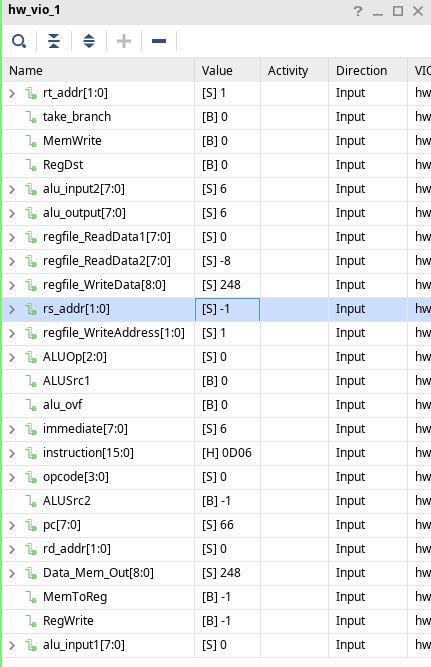
\includegraphics[width=\textwidth]{image}
	\caption{We got a -8! Visible in the regfile readData2, after loading the result from data memory.
		I should mention, the code is running 4 * -2. I'd love to test it with bigger numbers
		(bigger numbers will take the same number of instructions, cool enough) but I didn't have
		time (it's still a lot of instructions)}
\end{figure}



\end{document}
